\begin{frame}{Social pooling adds local motion context}
\textcolor{Teal}{\large WANG Yifan \quad Social-LSTM}
\begin{itemize}
\item Eight observed positions predict one twelve-step future.
\item A spatial grid pools neighbors' recurrent hidden states.
\item Closed-loop training and clean-validation ADE select the model.
\end{itemize}
\textbf{Shared evaluation:} 5 folds, 3 seeds, 15 training runs, $K=1$.
\par\medskip
{\footnotesize\color{Muted}Alahi et al., CVPR 2016. Declared deterministic adaptation. Local common-interface audit passed.}
\end{frame}
\begin{frame}{Shared evaluation separates accuracy and robustness}
\centering
\begin{tabular}{lr}\toprule
Predictor / input condition & ADE (m) \\\midrule
Constant velocity, clean, $K=1$ & 0.534 \\
Social-LSTM, clean, $K=1$ & \ModelMetric{social_lstm}{clean_0}{mean_ade_mean} \\
Social-LSTM, target noise 0.20\,m & \ModelMetric{social_lstm}{noise_020}{mean_ade_mean} \\
Social-LSTM, two missing positions & \ModelMetric{social_lstm}{missing_2}{mean_ade_mean} \\\bottomrule
\end{tabular}
\par\medskip
\small Constant velocity therefore remains the stronger aggregate baseline in this experiment.
\par\medskip
{\footnotesize\color{Muted}Identical shared test windows. Equal-scene macros, three seeds. One deterministic forecast per window.}
\end{frame}
\begin{frame}{A turning trajectory under target corruption}
\centering
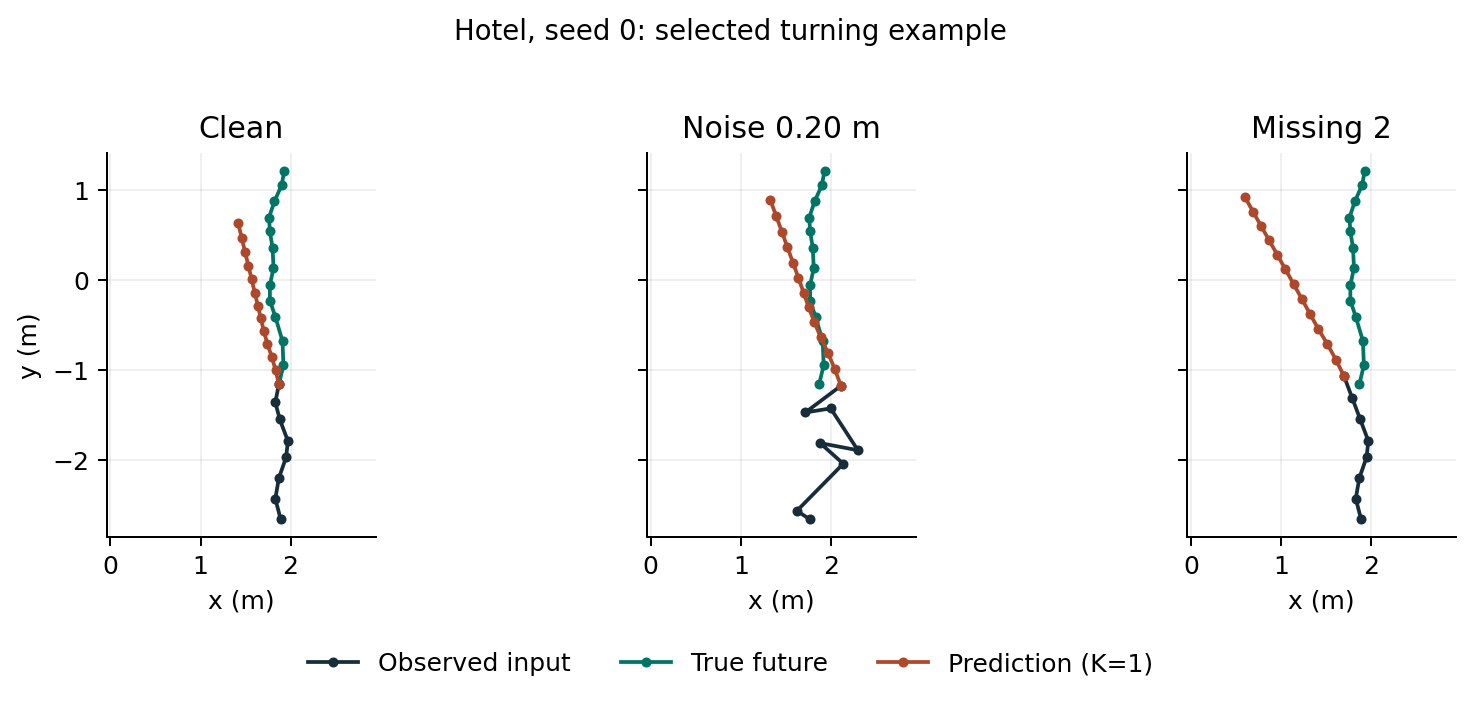
\includegraphics[height=.51\textheight,keepaspectratio]{contributions/social_lstm/evidence/causal_turning.png}
\par\smallskip
\small Same checkpoint and future. Only target observations change.
\par\medskip
{\footnotesize\color{Muted}Selected Hotel seed-0 example from fixed runtime IDs. Descriptive, not representative.}
\end{frame}
